\section{Introducción}
Este capítulo detalla el diseño técnico y arquitectónico del ``Asistente Virtual para la Preparación del Examen \gls{pmp}''. Se describe la estructura lógica y física del sistema, los componentes de software desarrollados, los modelos de datos implementados y los flujos de interacción que permiten el funcionamiento de las capacidades de \gls{ia} generativa. El diseño se ha orientado a crear una solución escalable, modular y mantenible, priorizando la experiencia del usuario y la precisión pedagógica.

\section{Arquitectura general del sistema}
La arquitectura del sistema ha sido diseñada siguiendo los principios modernos de la ingeniería de software para aplicaciones web, priorizando la velocidad, la seguridad y la facilidad de uso. Se ha adoptado un enfoque modular que separa claramente la interfaz visual con la que interactúa el usuario de la lógica de procesamiento y el almacenamiento de datos.

Esta separación permite que el sistema sea:
\begin{itemize}
\item \textbf{Rápido:} la interfaz carga casi instantáneamente, ofreciendo una experiencia fluida similar a una aplicación de escritorio.
\item \textbf{Escalable:} puede manejar un número creciente de estudiantes sin degradar su rendimiento, gracias al uso de servicios en la nube que se ajustan automáticamente a la demanda.
\item \textbf{Seguro:} los datos sensibles y la lógica de negocio están protegidos en servidores seguros, lejos del acceso directo del navegador del usuario.
\end{itemize}

\subsection{Diagrama de arquitectura de alto nivel}
El sistema se estructura en cuatro capas lógicas claramente diferenciadas, cada una con responsabilidades específicas:

\begin{enumerate}
\item \textbf{Capa de Presentación (interfaz de usuario):}
    es la cara visible del asistente. Se ejecuta en el navegador web del estudiante (Chrome, Edge, Firefox, etc.) y es responsable de mostrar la información de manera clara y atractiva. Gestiona la interacción directa, como hacer clic en botones, escribir en el chat o seleccionar respuestas en el simulador. Su diseño está optimizado para responder de inmediato a las acciones del usuario, evitando recargas innecesarias de la página.

\item \textbf{Capa de Aplicación y Lógica (cerebro del sistema):}
    actúa como intermediario entre lo que el usuario ve y los datos almacenados. Sus funciones principales incluyen:
    \begin{itemize}
    \item Verificar la identidad del usuario (seguridad).
    \item Procesar las solicitudes de estudio (por ejemplo, \enquote{iniciar un examen}).
    \item Coordinar la comunicación con la Inteligencia Artificial, enviando el contexto necesario para que las respuestas sean pertinentes y educativas.
    \end{itemize}

\item \textbf{Capa de Datos (memoria del sistema):}
    es el almacén seguro donde reside toda la información persistente. Aquí se guardan:
    \begin{itemize}
    \item Los perfiles y credenciales de los estudiantes.
    \item El historial de conversaciones con el asistente.
    \item El progreso detallado, incluyendo puntajes de exámenes y niveles completados.
    \end{itemize}
    Esta capa garantiza que, si el usuario cierra la sesión y vuelve otro día, todo su avance esté intacto.

\item \textbf{Capa de inteligencia cognitiva (motor de \gls{ia}):}
    Es el componente externo que dota de ``inteligencia'' al asistente. El sistema se conecta con un \gls{llm} (similar a los que impulsan herramientas como ChatGPT o Gemini) para generar explicaciones, analizar respuestas y crear escenarios de práctica en tiempo real.
\end{enumerate}

\begin{figure}[H]
\centering
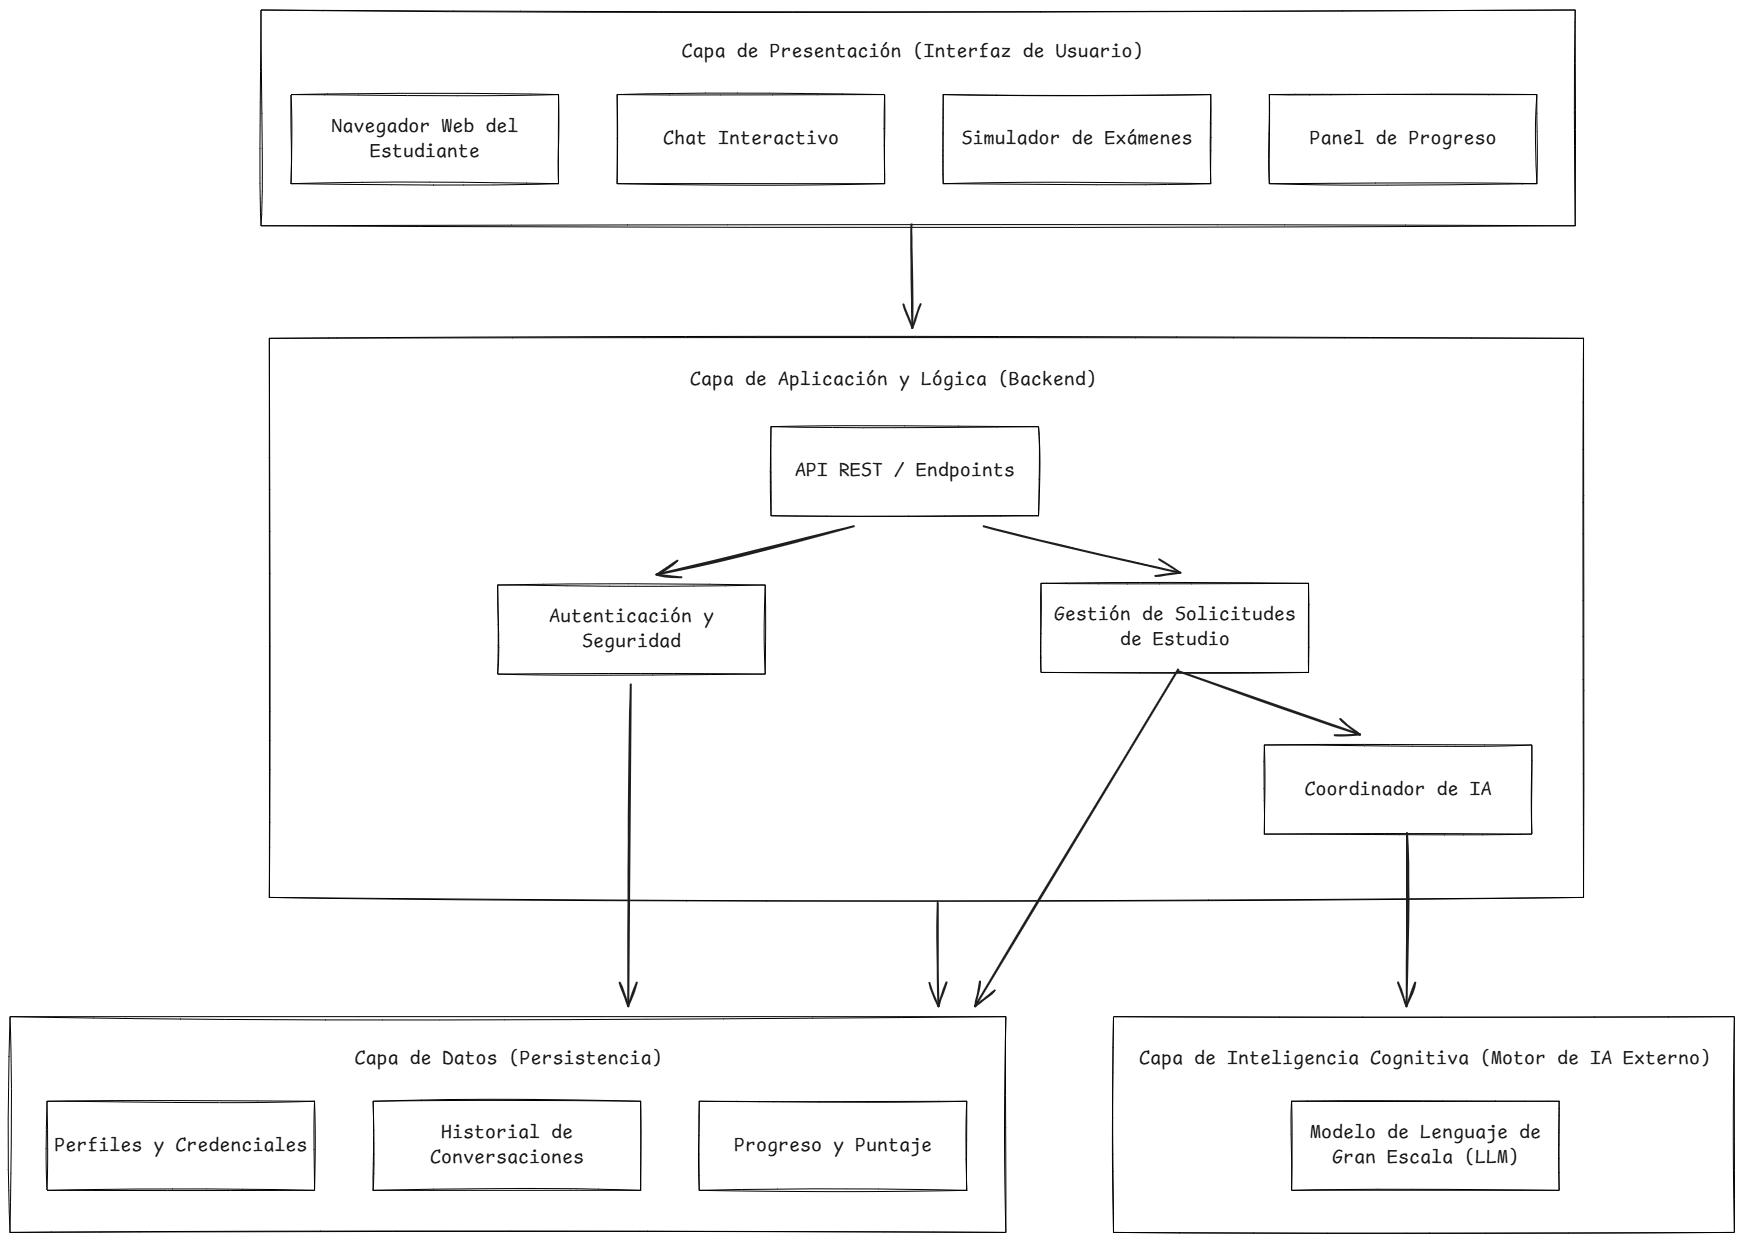
\includegraphics[width=1.0\textwidth]{figuras/diagrama_arquitectura_alto_nivel.png}
\caption{Diagrama de arquitectura de alto nivel.}
\label{fig:4-1}
\end{figure}

\subsection{Tecnologías utilizadas}
Para construir el asistente, se han seleccionado herramientas modernas y ampliamente probadas en la industria, priorizando la facilidad de mantenimiento y la experiencia del usuario.

\subsubsection{A. Desarrollo de la aplicación (frontend y lógica)}
\begin{itemize}
\item \textbf{Next.js y React:} son los cimientos sobre los que se construye la aplicación. Permiten crear interfaces web dinámicas que se sienten tan rápidas como una aplicación instalada en el ordenador. Su tecnología optimiza la carga de las páginas, asegurando que el estudiante pueda acceder al contenido rápidamente, incluso con conexiones a internet lentas.
\item \textbf{TypeScript:} es el lenguaje de programación utilizado. A diferencia de JavaScript estándar, TypeScript añade reglas estrictas que ayudan a prevenir errores comunes de programación antes de que la aplicación se ejecute, garantizando un software más robusto y fiable.
\end{itemize}

\subsubsection{B. Diseño visual e interactividad}
\begin{itemize}
\item \textbf{Tailwind CSS:} un sistema de diseño que permite crear interfaces limpias, modernas y que se adaptan automáticamente a cualquier tamaño de pantalla (celulares, tablets o computadoras de escritorio).
\item \textbf{Framer Motion:} una biblioteca especializada en animaciones. Se utiliza para suavizar las transiciones entre pantallas y dar feedback visual (como celebrar cuando se completa un nivel), haciendo que el estudio sea menos monótono y más interactivo.
\item \textbf{Iconografía (Lucide):} se emplea un conjunto de iconos estandarizados para facilitar la navegación intuitiva por la plataforma.
\end{itemize}

\subsubsection{C. Gestión de datos y conectividad}
\begin{itemize}
\item \textbf{PocketBase:} es el motor de base de datos. Se eligió por ser una solución compacta y extremadamente rápida, capaz de manejar miles de registros de estudiantes y simulaciones sin la complejidad de administración de las bases de datos corporativas tradicionales.
\item \textbf{LangChain:} actúa como un ``traductor'' o intermediario entre nuestra aplicación y la Inteligencia Artificial. Facilita el envío de instrucciones complejas a la IA y asegura que sus respuestas (ya sean texto, preguntas de examen o feedback) lleguen en el formato correcto para ser mostradas al estudiante.
\end{itemize}

\subsubsection{D. Motor de \gls{ia}}
\begin{itemize}
\item \textbf{Google Gemini 3.0 Flash:} es el cerebro cognitivo del asistente. Se seleccionó esta versión específica por su velocidad de respuesta (latencia ultra baja) y su capacidad para procesar grandes cantidades de información (como capítulos enteros del \gls{pmbok}) sin perder el hilo de la conversación (ver análisis comparativo y justificación técnica en Anexo \ref{anexo:seleccion_llm}).
\end{itemize}
\section{Componentes principales del asistente virtual}
El sistema se ha construido como un conjunto de piezas modulares (componentes) que funcionan de manera independiente pero coordinada. Esta estrategia facilita el mantenimiento y permite actualizar partes específicas del sistema sin afectar al resto.

\subsection{Estructura de la interfaz}

\subsubsection{A. Navegación y panel de control}
\begin{itemize}
\item \textbf{Barra lateral (sidebar):} es el menú de navegación principal. Se adapta automáticamente a dispositivos móviles (se oculta para ahorrar espacio) y gestiona la sesión del usuario, permitiendo cerrar sesión de forma segura y rápida.
\item \textbf{Panel principal (dashboard):} es el centro de mando del estudiante. Al iniciar sesión, este componente consulta en tiempo real el progreso del usuario y calcula sus estadísticas. Su diseño es flexible y permite alternar entre cuatro vistas principales:
    \begin{itemize}
    \item \textbf{Modo Guiado:} un mapa de progreso paso a paso, ideal para quienes estudian por primera vez. Bloquea temas avanzados hasta que se dominan los básicos.
    \item \textbf{Modo Desbloqueado:} permite acceso libre a todo el contenido, útil para repasos rápidos antes del examen.
    \item \textbf{Modo Libre:} un menú de herramientas especializadas (como simuladores de crisis o tutores de fórmulas) para uso a demanda.
    \item \textbf{Modo Simulación:} muestra el historial de exámenes y permite retomar simulacros interrumpidos.
    \end{itemize}
\end{itemize}

\begin{figure}[H]
\centering
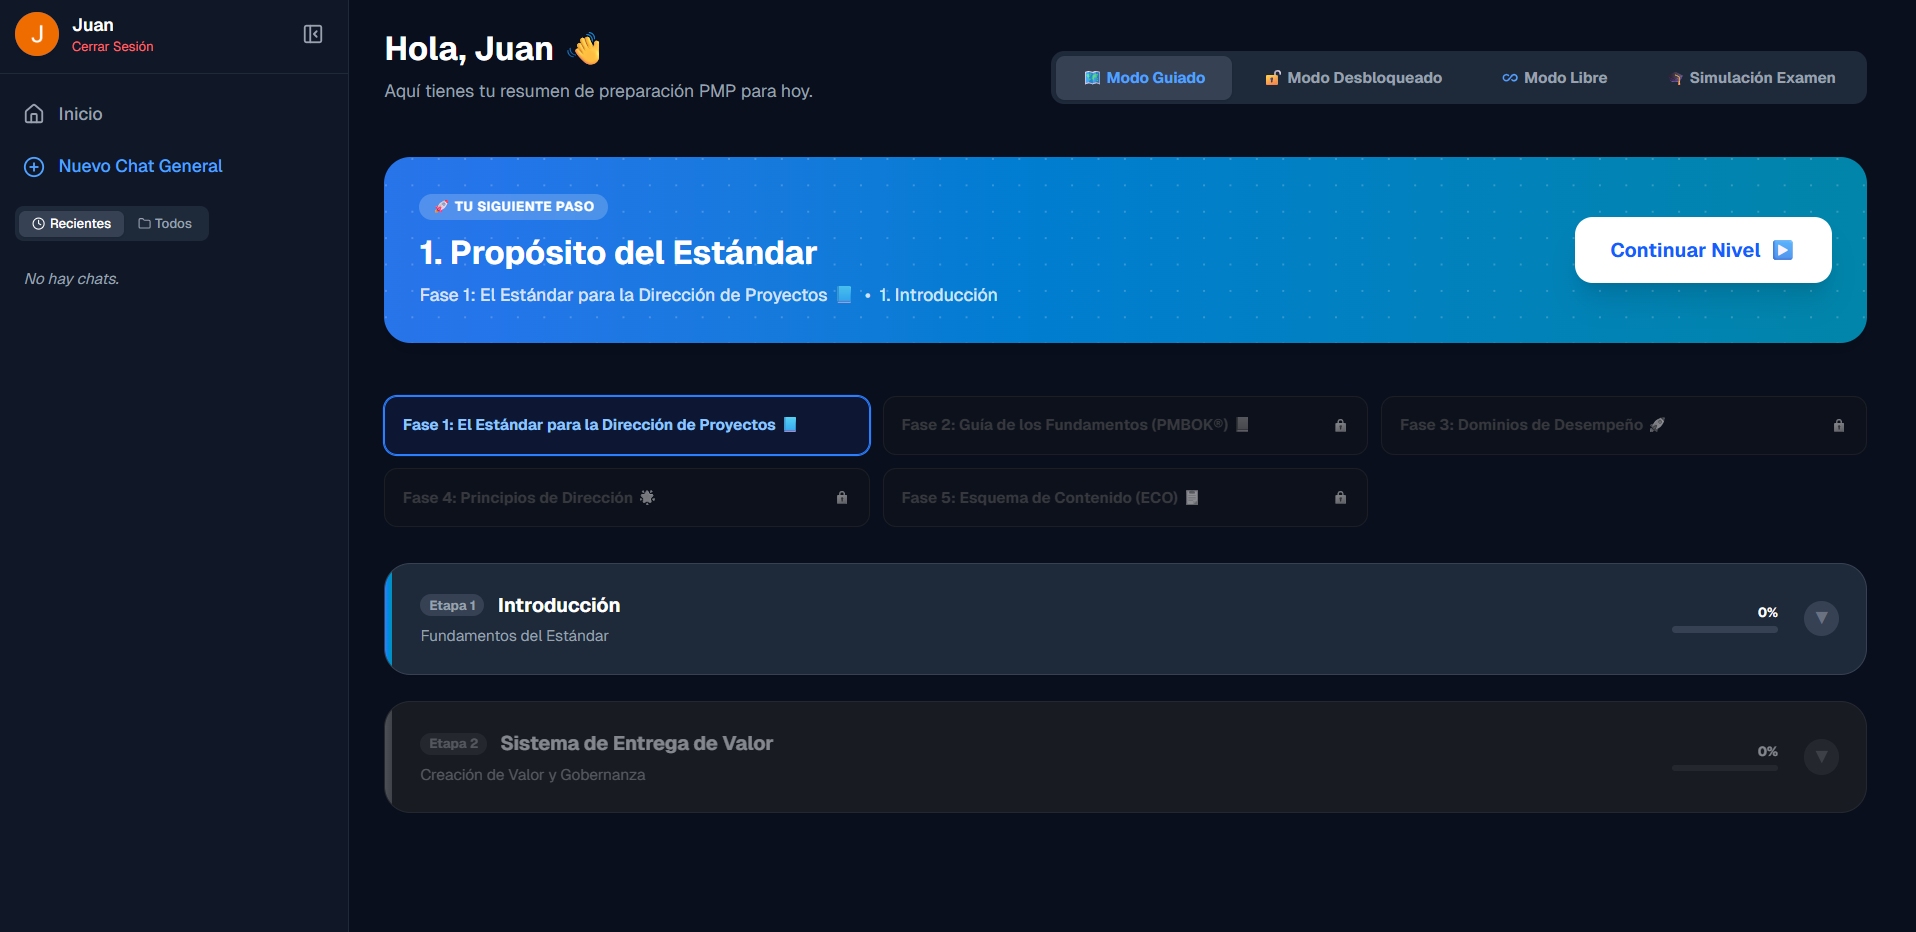
\includegraphics[width=1.0\textwidth]{figuras/navegacion_y_panel_de_control.png}
\caption{Navegación y panel de control.}
\label{fig:4-2}
\end{figure}

\subsubsection{B. El chat inteligente}
Este es el corazón de la interacción con el asistente. Se ha diseñado para que la conversación se sienta natural y fluida:
\begin{itemize}
\item \textbf{Escritura en tiempo real:} a diferencia de los sistemas antiguos que hacían esperar al usuario hasta tener la respuesta completa, este chat muestra la respuesta palabra por palabra a medida que la IA la genera (efecto ``streaming''), reduciendo la sensación de espera.
\item \textbf{Contexto adaptable:} el chat sabe en qué ``modo'' está el usuario. Si se selecciona el modo ``Socrático'', la IA no dará respuestas directas, sino que hará preguntas guía. Si se selecciona ``Simulación de Crisis'', actuará como un jefe exigente. Todo esto sucede sin necesidad de recargar la página.
\item \textbf{Formato rico:} las respuestas no son solo texto plano; pueden incluir tablas, listas, negritas y fragmentos de código, facilitando la lectura y el estudio.
\end{itemize}

\begin{figure}[H]
\centering
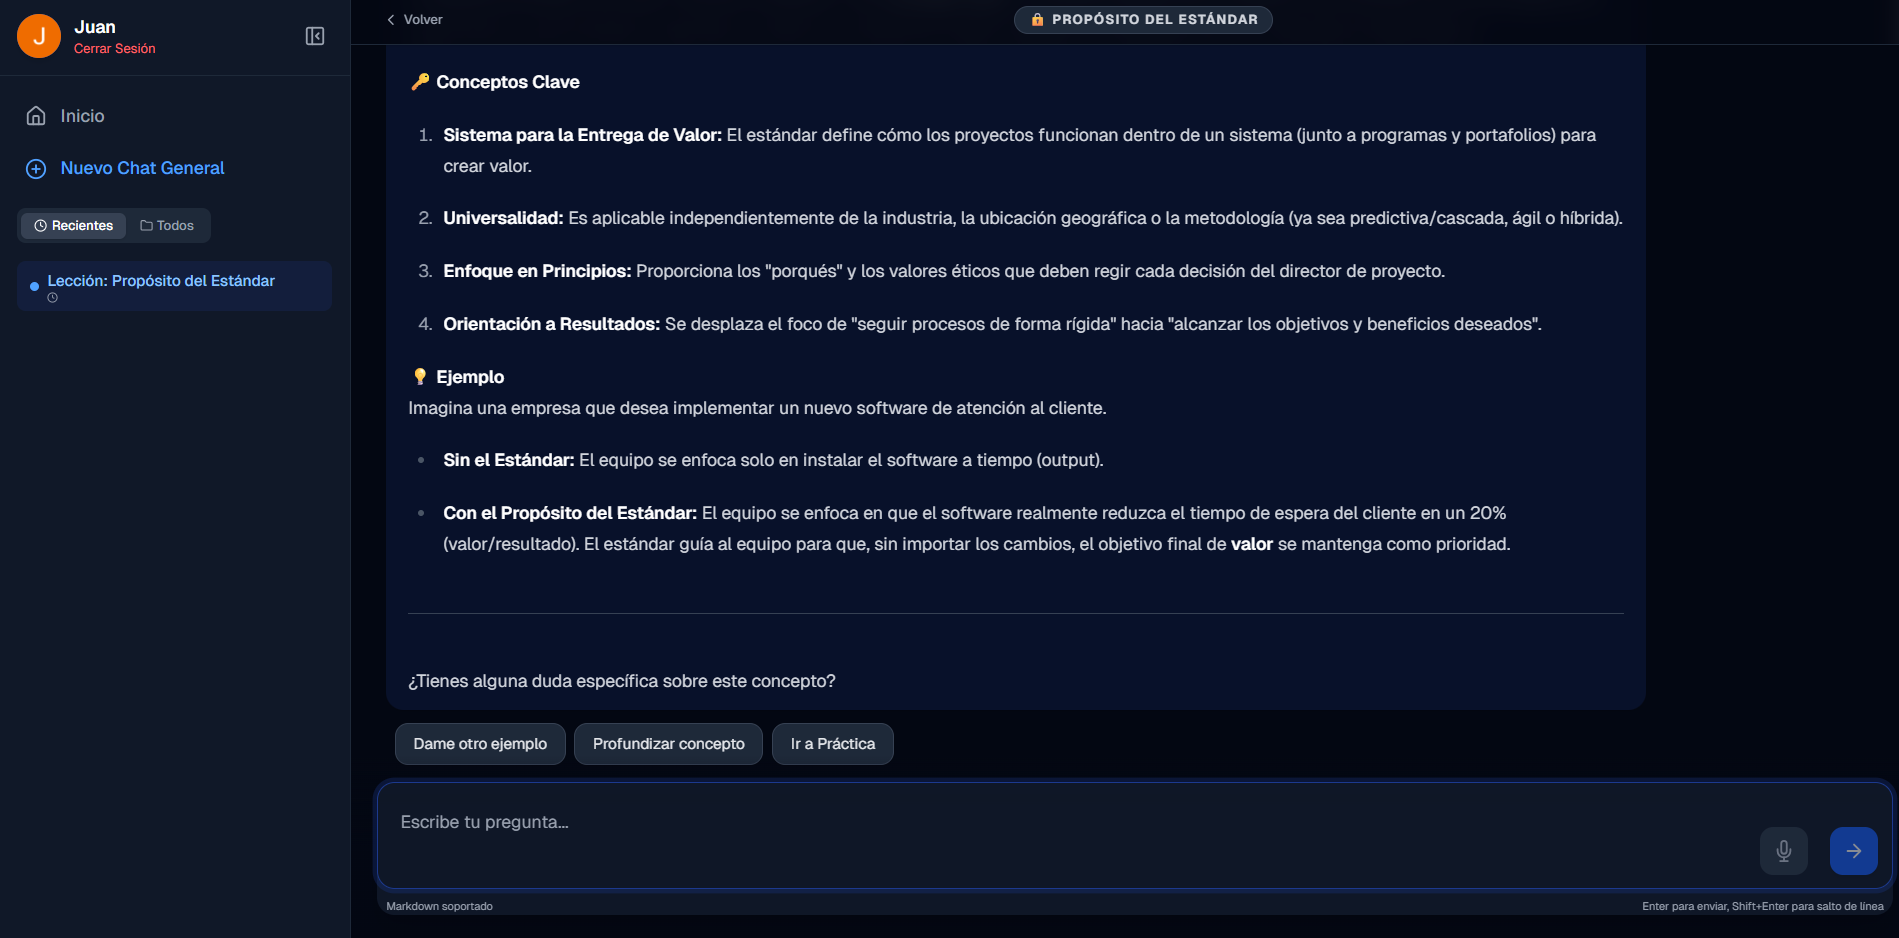
\includegraphics[width=1.0\textwidth]{figuras/el_chat_inteligente.png}
\caption{El chat inteligente.}
\label{fig:4-3}
\end{figure}

\subsubsection{C. Simulador de examen}
Este módulo recrea la presión y el formato del examen real \gls{pmp}:
\begin{itemize}
\item \textbf{Continuidad:} si el usuario pierde la conexión o cierra el navegador, el sistema guarda automáticamente el punto exacto donde se quedó.
\item \textbf{Carga inteligente:} para evitar esperas entre preguntas, el sistema utiliza una técnica de ``predicción'': mientras el usuario lee y responde la pregunta 1, el sistema ya está generando y preparando la pregunta 2 en segundo plano.
\item \textbf{Respuesta instantánea:} la interfaz reacciona inmediatamente al clic del usuario, dando una sensación de rapidez y fluidez.
\item \textbf{Feedback realista:} en el modo simulación, las explicaciones de las respuestas correctas solo se muestran al finalizar todo el examen, imitando las condiciones reales de la certificación.
\end{itemize}

\begin{figure}[H]
\centering
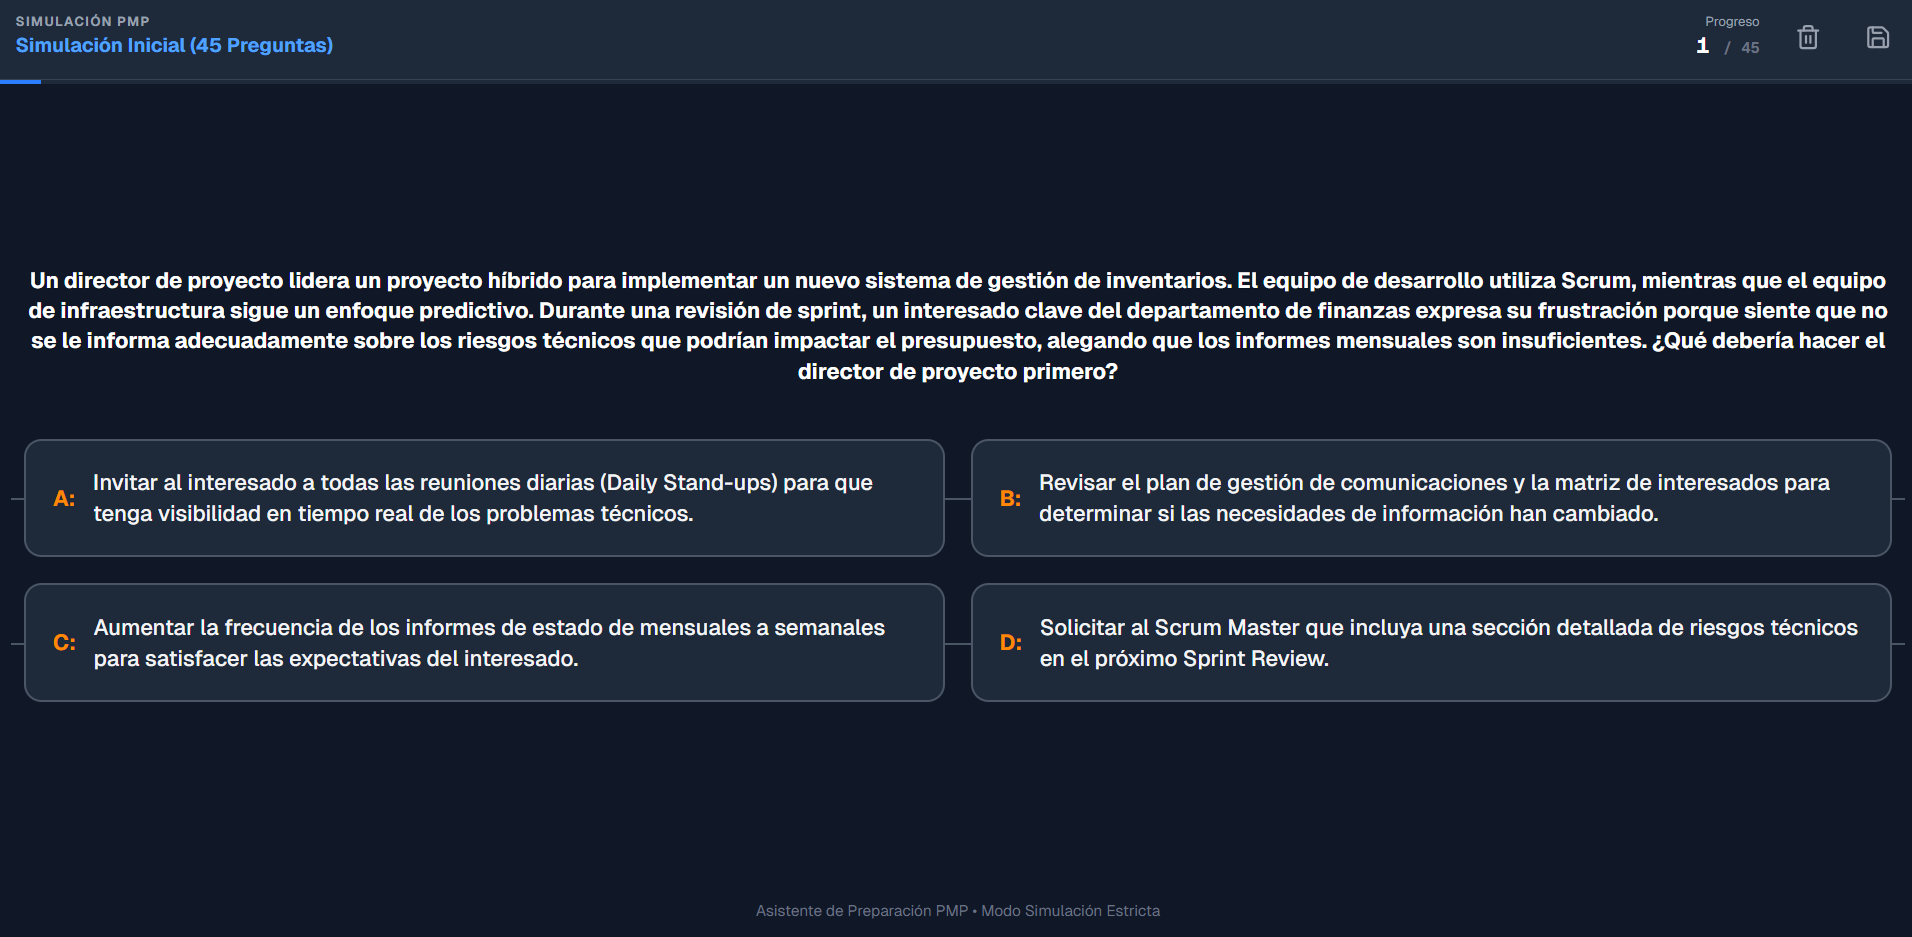
\includegraphics[width=1.0\textwidth]{figuras/simulador_de_examen.png}
\caption{Simulador de examen.}
\label{fig:4-4}
\end{figure}

\subsubsection{D. Elementos de ayuda y motivación}
\begin{itemize}
\item \textbf{Asistente de bienvenida:} una guía interactiva de 4 pasos que recibe a los nuevos usuarios, explicándoles cómo funciona la plataforma y cuál es la mejor estrategia de estudio.
\item \textbf{Sistema de logros:} pantallas de celebración animadas (con confeti y mensajes motivadores) que aparecen al completar un nivel, diseñadas para reforzar positivamente el avance del estudiante.
\end{itemize}

\begin{figure}[H]
\centering

\includegraphics[width=1.0\textwidth]{figuras/elementos_de_ayuda_y_motivacion.png}
\caption{Elementos de Ayuda y Motivación.}
\label{fig:4-5}
\end{figure}

\subsection{Estrategias de navegación y modos de estudio}
El dashboard principal actúa como un controlador de estado que adapta la experiencia de aprendizaje a través de cuatro modos de visualización distintos. Esta flexibilidad permite que la aplicación sirva tanto a estudiantes novatos que necesitan estructura como a expertos que buscan práctica específica.

\begin{enumerate}
    \item \textbf{Modo Guiado (gamificado):}
    \begin{itemize}
        \item \textbf{Enfoque:} progresión estructurada por niveles.
        \item \textbf{Comportamiento:} es la vista predeterminada. El contenido se organiza en ``Mundos'' temáticos que se desbloquean secuencialmente. Cada nivel ofrece cuatro tipos de interacción especializada con la IA:
        \begin{itemize}
            \item \textbf{Lección magistral (El Gran Bibliotecario):} entrega explicaciones estructuradas con definiciones, ejemplos y conceptos clave sobre el tema específico del nivel.
            \item \textbf{Entrenamiento práctico (El Entrenador de Combate):} presenta escenarios breves y situaciones prácticas donde el usuario debe aplicar lo aprendido inmediatamente.
            \item \textbf{El Oráculo (consultas del nivel):} un asistente experto limitado exclusivamente al tema del nivel actual, ideal para resolver dudas específicas sin desviarse del objetivo de aprendizaje.
            \item \textbf{Prueba de fuego (El Guardián):} un examen corto y riguroso (generalmente 3 preguntas) que el usuario debe aprobar para demostrar su dominio del tema y desbloquear el siguiente nivel.
        \end{itemize}
        \item \textbf{Objetivo:} garantizar que el estudiante construya su conocimiento sobre bases sólidas, alternando teoría, práctica, consulta y evaluación antes de avanzar.
    \end{itemize}

    \item \textbf{Modo Desbloqueado:}
    \begin{itemize}
        \item \textbf{Enfoque:} referencia y consulta.
        \item \textbf{Comportamiento:} utiliza la misma interfaz visual de mapas y mundos que el Modo Guiado, pero elimina todas las restricciones de acceso. Todos los niveles son accesibles instantáneamente.
        \item \textbf{Objetivo:} permitir a usuarios avanzados o repetidores navegar libremente para reforzar áreas específicas sin la fricción de tener que ``desbloquear'' contenido ya conocido.
    \end{itemize}

    \item \textbf{Modo Libre:}
    \begin{itemize}
        \item \textbf{Enfoque:} herramientas de \gls{ia} a la carta.
        \item \textbf{Comportamiento:} reemplaza completamente la visualización del mapa de niveles por un menú de tarjetas. Ofrece herramientas especializadas diseñadas para cubrir diferentes estilos de aprendizaje:
        \begin{itemize}
            \item \textbf{Modo Estándar:} el asistente clásico. Proporciona preguntas y respuestas directas sobre cualquier tema del \gls{pmbok}.
            \item \textbf{Simulación de Crisis:} un roleplay inmersivo donde la \gls{ia} actúa como un stakeholder difícil.
            \item \textbf{Taller de Entregables:} ayuda al usuario a redactar documentos clave como el Project Charter.
            \item \textbf{Examen Rápido:} genera una serie corta de preguntas tipo \gls{pmp} con feedback inmediato.
            \item \textbf{Tutor Socrático:} la \gls{ia} guía al usuario mediante preguntas reflexivas en lugar de dar respuestas directas.
            \item \textbf{Debate (Abogado del Diablo):} la \gls{ia} adopta una postura polémica que el usuario debe refutar con argumentos técnicos y éticos.
            \item \textbf{Caso de Estudio:} escenarios complejos para diagnosticar problemas raíz y proponer planes de acción.
            \item \textbf{Explícamelo como a un niño:} simplifica conceptos densos utilizando analogías cotidianas.
            \item \textbf{Entrenador de Fórmulas:} ejercicios prácticos sobre \gls{evm}\glsadd{evm}, \gls{cpm}\glsadd{cpm} y proyecciones financieras.
        \end{itemize}
        \item \textbf{Objetivo:} Ofrecer acceso directo a las capacidades del \gls{llm} fuera del contexto de un ``nivel'' específico.
    \end{itemize}

    \item \textbf{Simulación Examen:}
    \begin{itemize}
        \item \textbf{Enfoque:} evaluación y métricas.
        \item \textbf{Comportamiento:} transforma el dashboard en un centro de análisis de datos. Muestra gráficos de rendimiento acumulado y permite lanzar simulacros de 45 a 180 preguntas.
        \item \textbf{Objetivo:} validar la preparación del estudiante bajo condiciones controladas y proporcionar feedback cuantitativo.
    \end{itemize}
\end{enumerate}
\subsection{Servicios de backend (lógica del servidor)}
Aunque invisibles para el usuario, estos servicios son los encargados de que todo funcione correctamente.

\subsubsection{A. Servicio de chat}
Este servicio gestiona la conversación con la \gls{ia}. Sus tareas principales son:
\begin{itemize}
\item \textbf{Verificación:} se asegura de que los mensajes sean válidos y provengan de un usuario autorizado.
\item \textbf{Conexión con la \gls{ia}:} envía la conversación al modelo de Google Gemini, añadiendo instrucciones especiales según el modo de estudio elegido (por ejemplo, \enquote{actúa como un profesor socrático} o \enquote{actúa como un examinador estricto}).
\item \textbf{Entrega rápida:} envía la respuesta al usuario poco a poco, tal como la va generando la \gls{ia}, para que la conversación sea fluida.
\end{itemize}

\subsubsection{B. Generador de simulaciones}
Este es un componente crítico que permite crear exámenes infinitos.
\begin{itemize}
\item \textbf{Instrucciones precisas:} el sistema le pide a la \gls{ia} que cree preguntas con un formato muy específico (pregunta, opciones, respuesta correcta y explicación), asegurando que siempre se puedan mostrar correctamente en la pantalla.
\item \textbf{Control de calidad:} antes de mostrar las preguntas al usuario, el sistema revisa que tengan el formato correcto para evitar errores visuales.
\end{itemize}

\subsection{Modelo de datos (almacenamiento)}
La base de datos está organizada para guardar la información de manera eficiente y segura.

\begin{table}[H]
\centering
\small
\renewcommand{\arraystretch}{1.3}
\begin{tabularx}{\textwidth}{p{2.5cm} X}
\toprule
\textbf{Tipo de dato} & \textbf{Descripción} \\
\midrule
\textbf{Usuarios} & Guarda la información básica del estudiante (nombre, correo) y sus preferencias visuales. \\
\midrule
\textbf{Progreso} & Registra el avance del estudiante: nivel actual, racha de días estudiados y última fecha de acceso. \\
\midrule
\textbf{Chats} & Almacena el historial de todas las conversaciones para que el usuario pueda revisarlas más tarde. \\
\midrule
\textbf{Mensajes} & Guarda cada pregunta y respuesta individual dentro de una conversación. \\
\midrule
\textbf{Simulaciones} & Archiva los exámenes completos, incluyendo las preguntas generadas, las respuestas del usuario y la puntuación final. \\
\bottomrule
\end{tabularx}
\vspace{0.5em}
\caption{Estructura de la información almacenada}
\label{tab:4-1}
\end{table}

\begin{itemize}
\item \textbf{Privacidad y seguridad:}
    el sistema cuenta con reglas estrictas que garantizan que cada estudiante solo pueda ver y modificar sus propios datos. Nadie puede acceder al progreso o historial de otro usuario.
\end{itemize}

\section{Flujos de interacción y procesos}
A continuación se describe paso a paso cómo funcionan las características más importantes del sistema desde la perspectiva del usuario.

\subsection{Acceso y bienvenida}
\begin{enumerate}
\item \textbf{Verificación:} cuando un usuario intenta entrar, el sistema comprueba si ya ha iniciado sesión. Si no, lo redirige a la página de bienvenida.
\item \textbf{Inicio de sesión:} el usuario introduce sus datos. El sistema verifica la contraseña de forma segura y, si es correcta, le da acceso.
\item \textbf{Primera vez:} si es un usuario nuevo, se le muestra una guía interactiva (Onboarding) de 4 pasos para enseñarle a usar la plataforma.
\end{enumerate}

\subsection{Interacción con el chat}
\begin{enumerate}
\item \textbf{El usuario pregunta:} el estudiante escribe su duda y pulsa enviar. La interfaz muestra el mensaje inmediatamente para que se sienta rápido.
\item \textbf{El sistema procesa:} la aplicación envía el mensaje y el historial de la conversación a la Inteligencia Artificial, indicándole el \enquote{rol} que debe asumir (profesor, examinador, etc.).
\item \textbf{La \gls{ia} Responde:} la respuesta se muestra en pantalla progresivamente, como si alguien la estuviera escribiendo en ese momento. Una vez completa, se guarda en el historial.
\end{enumerate}

\subsection{Simulación de examen}
Este proceso es clave para la preparación del estudiante.
\begin{enumerate}
\item \textbf{Configuración:} el usuario elige el tema (ej. \enquote{Riesgos}) y la cantidad de preguntas.
\item \textbf{Generación:} la \gls{ia} crea un examen único y personalizado para esa sesión.
\item \textbf{Realización:} el estudiante responde las preguntas una a una. El sistema guarda sus respuestas automáticamente.
\item \textbf{Evaluación:} al terminar, el sistema calcula la nota, muestra qué respuestas fueron correctas e incorrectas, y ofrece explicaciones detalladas para aprender de los errores.
\end{enumerate}

\section{Decisiones de diseño y justificación}

Esta sección explica el \enquote{por qué} de las decisiones técnicas más importantes, enfocándose en cómo benefician al estudiante.

\subsection{Selección de la \gls{ia} (Google Gemini 3.0)}
Se eligió este modelo específico por cuatro razones clave:
\begin{enumerate}
\item \textbf{Gran memoria:} puede recordar toda la conversación y grandes partes del manual \gls{pmbok} sin olvidar el contexto.
\item \textbf{Velocidad:} responde casi al instante, lo cual es vital para mantener la concentración del estudiante.
\item \textbf{Capacidad de razonamiento:} es capaz de explicar el \enquote{por qué} de una respuesta, no solo decir si es correcta o falsa.
\item \textbf{Eficiencia:} permite ofrecer un servicio de alta calidad a muchos estudiantes sin costes prohibitivos.
\end{enumerate}

\subsection{Personalidad adaptable del asistente}
En lugar de tener un único \enquote{bot}, el sistema cambia de personalidad según lo que el estudiante necesite:
\begin{itemize}
\item \textbf{Modo Profesor:} explica conceptos con paciencia.
\item \textbf{Modo Socrático:} responde con preguntas para hacer pensar al estudiante.
\item \textbf{Modo Simulador:} actúa como un interesado (stakeholder) difícil en un proyecto real.
\end{itemize}

\subsection{Diseño centrado en el estudiante}
La interfaz se diseñó para minimizar distracciones:
\begin{itemize}
\item \textbf{Limpieza visual:} menús que se ocultan cuando no se necesitan.
\item \textbf{Modo oscuro:} para no cansar la vista en sesiones largas.
\item \textbf{Respuesta inmediata:} el sistema confirma cada acción del usuario al instante para dar sensación de control.
\end{itemize}
\subsection{Arquitectura de datos híbrida}
Se diseñó un modelo de datos híbrido que combina la inmutabilidad de los estándares educativos con la flexibilidad del progreso del usuario.

\begin{itemize}
\item \textbf{Contenido estático en código:} La estructura del \gls{pmbok} (dominios, tareas y principios) se codifica directamente en el cliente para garantizar acceso instantáneo y tipado estático.
\item \textbf{Datos dinámicos en PocketBase:} Solo los datos generados por el usuario se persisten en la base de datos, separando claramente la lógica de dominio del estado del usuario.

\end{itemize}
\subsection{Enfoque de gamificación estructural}
La gamificación se integró en el núcleo de la navegación.

\begin{itemize}
\item \textbf{Progresión bloqueada:} El usuario debe ``conquistar'' conceptos para desbloquear los siguientes, asegurando una ruta de aprendizaje coherente.
\item \textbf{Sistema de celebración:} Las modales de ``Nivel Completado'' (\texttt{LevelCompletedModal}) utilizan recompensas visuales (confeti) para motivar al usuario a completar sus objetivos diarios.

\end{itemize}
\section{Consideraciones de seguridad y robustez}

La seguridad en el desarrollo de software educativo garantiza la integridad del proceso de aprendizaje.

\subsection{Gestión segura de credenciales}
Las claves de la \gls{api} sensibles (\texttt{GOOGLE\_API\_KEY}) se almacenan en variables de entorno del lado del servidor, nunca expuestas al cliente. Next.js garantiza este aislamiento por diseño.

\subsection{Validación de datos y prevención de inyecciones}
\begin{itemize}
\item \textbf{Validación de esquema:} todas las entradas a los endpoints \gls{api} se validan rigurosamente (aunque el código actual utiliza validación manual y tipos TypeScript, la arquitectura está preparada para esquemas Zod).
\item \textbf{Sanitización:} se verifica la estructura de los \gls{json} generados por la IA antes de renderizarlos.

\end{itemize}
\subsection{Aislamiento de datos multi-inquilino}
Se implementa \gls{rls} en PocketBase:
\begin{itemize}
\item \texttt{user\_id = @request.auth.id}: regla inmutable que asegura que cada estudiante solo acceda a sus propios datos, independientemente de la lógica del frontend.

\end{itemize}
\subsection{Privacidad}
El sistema minimiza la recolección de datos, almacenando solo lo necesario para la continuidad pedagógica y el seguimiento del progreso.